\documentclass[hyperref={dvipdfmx,pdfpagelabels=false}]{beamer}
\title{Einführung in Matlab - Einheit 1}
\subtitle{Streifzug durch Matlab, Vektoren und Matrizen}
\mode<article>
{
  \usepackage{fullpage}
  \usepackage{pgf}
  \usepackage{hyperref}
  \setjobnamebeamerversion{beamer}
}

\mode<presentation>
{
  %\usetheme{Frankfurt}
 %\usetheme{My}
  \usetheme{Madrid}
  % or ...
%\usecolortheme{seagull}
  %\setbeamercovered{transparent}
  %\setbeamercovered{dynamic}
  % or whatever (possibly just delete it)
}
\usenavigationsymbolstemplate{}
\usefonttheme{structurebold}
\usepackage{multimedia}
\usepackage{tikz}
\usepackage{fontspec,xunicode,xltxtra}
%\usepackage[scaled=.90]{helvet}
% Or whatever. Note that the encoding and the font should match. If T1
% does not look nice, try deleting the line with the fontenc.

\setbeamertemplate{footline}
{
\leavevmode
%\hbox{\begin{beamercolorbox}[wd=.5\paperwidth,ht=2.5ex,dp=1.125ex,
%leftskip=.3cm plus1fill,rightskip=.3cm]{author in head/foot}%
%    \usebeamerfont{author in head/foot}\insertshortauthor
%  \end{beamercolorbox}%
%  \begin{beamercolorbox}[wd=.5\paperwidth,ht=2.5ex,dp=1.125ex,leftskip=.3cm,
%rightskip=.3cm plus1fil]{title in head/foot}%
%    \usebeamerfont{title in head/foot}\insertshorttitle\hfill

\hfill\insertframenumber  \hspace{3pt}

%\inserttotalframenumber
%\hspace*{2ex}
%  \end{beamercolorbox}}%
  \vskip3pt%
}

%\usepackage[english]{babel}
\usepackage[ngerman]{babel}
\selectlanguage{ngerman}

%
% math/symbols
%
\usepackage{amssymb}
\usepackage{amsthm}
% \usepackage{latexsym}
\usepackage{amsmath}
%\usepackage{listings}
\usepackage[framed]{mcode}
%\usepackage{mcode}

\usepackage{mydef}
\usepackage{cmap} % you can search in the pdf for umlauts and ligatures
%\usepackage{colonequals} %corrects the definition-symbols \colonequals (besides others)
\title{Einführung in Matlab}
%
%\subtitle{Disputation} % (optional)

\author{Jochen Schulz}
% - Use the \inst{?} command only if the authors have different
%   affiliation.

\institute{Georg-August Universit\"at G\"ottingen \pgfimage[height=0.5cm]{../figures/unilogo3}}
% - Use the \inst command only if there are several affiliations.
% - Keep it simple, no one is interested in your street address.

\date{\today}

\subject{Einführung in Matlab}
% This is only inserted into the PDF information catalog. Can be left
% out. 



% If you have a file called "university-logo-filename.xxx", where xxx
% is a graphic format that can be processed by latex or pdflatex,
% resp., then you can add a logo as follows:

%\logo{\pgfimage[height=0.5cm]{figures/unilogo3}}


% Delete this, if you do not want the table of contents to pop up at
% the beginning of each subsection:
% \AtBeginSubsection[]
% {
%   \begin{frame}<beamer>
%     \frametitle{Aufbau}
%     \tableofcontents[currentsection,currentsubsection]
%   \end{frame}
% }

\AtBeginSection[]
{
  \begin{frame}<beamer>
    \frametitle{Aufbau}
    \tableofcontents[currentsection,currentsubsection]
  \end{frame}
}


\begin{document}



\maketitle


\begin{frame}{Organisatorisches}
\begin{itemize}
\item Anmeldung über StudIP \\
      \url{https://www.studip.uni-goettingen.de/}

{\color{blue}{Einführung in Matlab (Mathematische Anwendersysteme)}}
\item Alle Unterlagen (Aufgabenblätter, Vorlesungsfolien, Beispiele, Musterlösungen) $\rightarrow$ StudIP
\pause
\begin{block}{Dozent}
Jochen Schulz\\
NAM, Zimmer 04 (Erdgescho{\ss})\\
\textbf{Telefon}: 39-4525\\
\textbf{Email}: \href{mailto:schulz@math.uni-goettingen.de}{\texttt{schulz@math.uni-goettingen.de}}\\
\textbf{XMPP}: \url{schulz@jabber.num.math.uni-goettingen.de}\\

\end{block}
\end{itemize}
\end{frame}

\begin{frame}{Ablauf der Veranstaltung}
\begin{itemize}
\item Blockveranstaltung vom  12.9 - 23.9.2011
\item \alert{Vorlesung:} 9.15 - 11.30  (MN )
\item \alert{Übungsbetrieb/Praktikum}: 13:00 - 18:00  (MM-Raum oder NAM-CIP)
\begin{itemize}
\item 1 Übungszettel/Tag.
\item Besprechung Aufgaben vom Vortag
\item Hilfestellung beim Bearbeiten der aktuellen Aufgaben
%\item Klausurzulassung: 3 beliebige markierte Aufgaben/Woche testieren lassen. 
\end{itemize}
\item \alert{Klausur:} 30.9.2011 (?); 10:00 - 11:30; Anmeldung über FlexNow.
\end{itemize}

\end{frame}

\begin{frame}{Inhalt der Vorlesung}
\begin{description}
 \item[1. Tag] Organisatorisches, Streifzug durch Matlab
\item [2. Tag] Programmieren, Datenstrukturen
\item [3. Tag] Rekursionen, Grafik
\item [4. Tag] Polynome, Interpolation, Visualisieren, Debugging
\item [5. Tag] Mehrdimensionale Arrays, Funktionen, Numerische Lineare Algebra, Dünnbesetzte Matrizen
\item [6. Tag] Numerische Mathematik ?%profiler?, objektorientierung?
\item [7. Tag] Grafik-Handle, GUIs
\item [8. Tag] Schnittstelle zu C
\item [9. Tag] Wunschvorlesung
\item [10. Tag] Fragestunde
\end{description}
\end{frame}

\begin{frame}{Aufbau}
\tableofcontents
\end{frame}

\section{Streifzug durch MATLAB}

\subsection{Einleitung}
%-------------------------------------------------
%  Folie:
%-------------------------------------------------
\begin{frame}[fragile]\frametitle{MATLAB}

\begin{itemize}
\item MATLAB steht für \alert{Mat}rix \alert{lab}oratory; ursprünglich speziell Matrizenrechnung.
\item Entwickelt von Cleve Moler Ende der 70'er in FORTRAN.
\item Heutige Version ist in C/C++ programmiert.
\item Interaktives System für numerische Berechnungen und Visualisierungen.
\item Kein Computer-Algebra-System (Aber erweiterbar durch \texttt{symbolic math toolbox})
\end{itemize}
\end{frame}

%-------------------------------------------------
%  Folie:
%-------------------------------------------------
\begin{frame}[fragile]\frametitle{Vorteile von MATLAB}

\begin{itemize}
\item \emph{High-Level} Sprache:
\begin{itemize}
\item Programmieren ist leicht (aber auch beschränkt(er))
\item Schnelle Erfolge 
\item Sehr geeignet für Prototyping und Debugging
\end{itemize}
\item Vielfältige Visualisierungsmöglichkeiten.
\item MATLAB-Programme sind vollständig portierbar zwischen Architekturen (cross-plattform).
\item zusätzliche Toolboxes (Symb. Math T., PDE T., Wavelet T.)  
\item Ausgereifte Oberfläche.
\end{itemize}
\end{frame}

%-------------------------------------------------
%  Folie:
%-------------------------------------------------
\begin{frame}[fragile]\frametitle{Literatur}
\begin{thebibliography}{10}
\small
\bibitem{1} Matlab online-help :-).
\bibitem{2}
\alert{Matlab Guide}, D.J. Higham, N.J. Higham, SIAM, 2000, 
\bibitem{3} \alert{Introduction to Scientific Computing}, C.F. van Loan, Prentice Hall,
New Jersey, 1997,
\bibitem{4} \alert{Scientific Computing with MATLAB}, A. Quarteroni, F. Saleri, Springer, 2003,
\bibitem{5} \alert{Graphics and GUIs with MATLAB}, P. Marchand, O.Th. Holland, Chapman \& Hall, 2003, 3. Aufl.
\bibitem{6} \alert{MATLAB 7}, C. \"Uberhuber, St. Katzenbeisser, D. Praetorius, Springer 2005.
\bibitem{7} \alert {Using \textsc{Matlab}}, offizielle Handbücher.
\end{thebibliography}
\end{frame}


\subsection{Grundlegende Bedienung}
%-------------------------------------------------
%  Folie:
%-------------------------------------------------
\begin{frame}[fragile]\frametitle{MATLAB Fenster-Aufbau}
Starten von MATLAB: Eingabe von \mcode{matlab &} (in einem Terminal).
\centering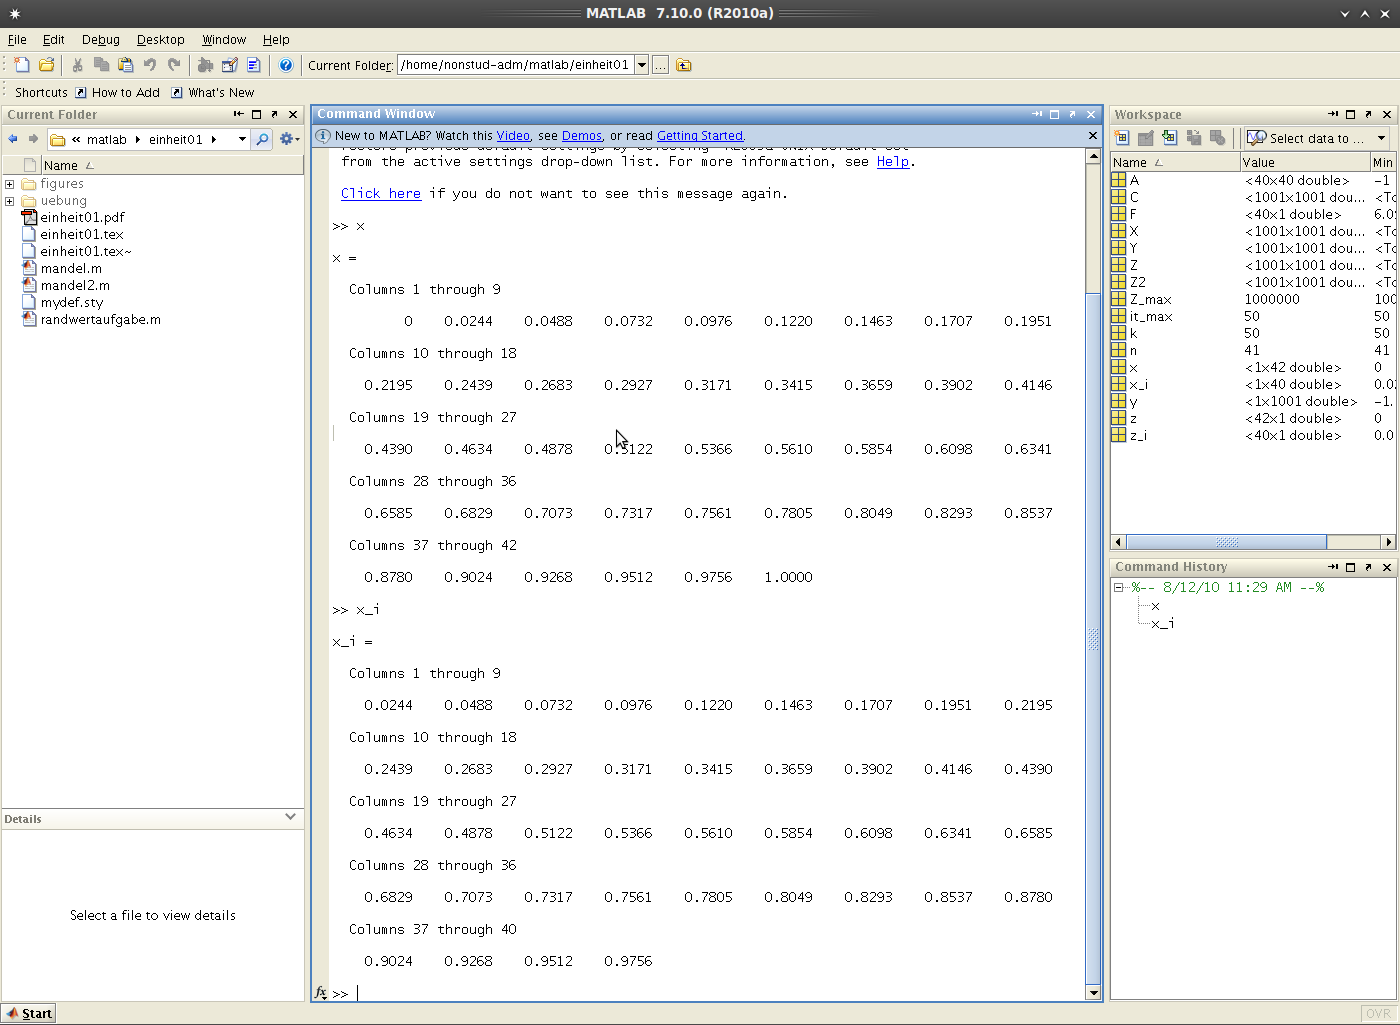
\includegraphics[width=0.55\textwidth]{figures/Screenshot-MATLAB}

\begin{columns}[c]
\column{0.48\textwidth}
\begin{itemize}
\item \alert{Launch Pad:} Startmenü
\item \alert{Command Window:} Befehlseingabe und Standardausgabe
\end{itemize}
\column{0.48\textwidth}
\begin{itemize}
\item \alert{Workspace:} Ansicht von Variablen und deren Art und Grösse; Ändern der
Einträge 
\item \alert{Grafik:} normalerweise in separaten Fenstern
\end{itemize}

\end{columns}
\end{frame}

%-------------------------------------------------
%  Folie:
%-------------------------------------------------
\begin{frame}[fragile]\frametitle{Command Window - Befehle }
\begin{itemize}
\item Erster Befehl
\begin{lstlisting}
>> 2+2
ans = 4
\end{lstlisting}
%\item Variable \mcode{ans} jetzt im Workspace.
\item Editieren alter Eingaben:  $\uparrow$, $\downarrow$ (wie
in Unix)
%\item aktuelles Verzeichnis: \mcode{pwd}
\item Mit \mcode{;} am Ende jeder Befehlszeile wird Standardausgabe unterdrückt.
\begin{lstlisting}
>> 2+2;
\end{lstlisting}
\item Hilfe zu Befehlen: \mcode{help <command>} oder \mcode{doc <command>}
\item Zuweisung 
\begin{lstlisting}
>> a = 2+2;
\end{lstlisting}
\item Funktionsaufruf 
\begin{lstlisting}
>> sin(2)
ans = 0.9093
\end{lstlisting}
\item Verlassen von MATLAB: \mcode{quit} oder \mcode{exit}
\end{itemize}
\end{frame}


%-------------------------------------------------
%  Folie:
%-------------------------------------------------
\begin{frame}[fragile]\frametitle{Workspace - globale Variablen}
\begin{itemize}
\item Alle definierten (globalen) Variablen werden im Workspace gespeichert.
\item Zugriff während einer MATLAB-Sitzung.
\item Inhalt des Arbeitsspeichers: \mcode{whos} oder \mcode{who}
\begin{lstlisting}
>> whos
  Name      Size            Bytes  Class   

  ans       1x1                 8  double    
\end{lstlisting}
\item Löschen von Variablen : \mcode{clear <var>};\\
\mcode{clear} löscht den gesamten Arbeitsspeicher (Workspace).
\end{itemize}
\end{frame}




\subsection{Erste Schritte}
%-------------------------------------------------
%  Folie:
%-------------------------------------------------
\begin{frame}[fragile]\frametitle{Erste Schritte}
\begin{itemize}
\item MATLAB als Taschenrechner \newline (Ergebnis wird in \mcode{ans} gespeichert.) 
\begin{lstlisting}
>> 1+(sin(pi/2)+ exp(2))*0.5
ans = 5.1945
\end{lstlisting}
\item Eingabe von (Zeilen-)Vektoren
\begin{lstlisting}
>> x = [1 2 3]  
\end{lstlisting}
\item Transponieren und speichern in  Variable \mcode{b}
\begin{lstlisting}
>> b = transpose(x)
\end{lstlisting}
\end{itemize}
\end{frame}

%-------------------------------------------------
%  Folie:
%-------------------------------------------------
\begin{frame}[fragile]\frametitle{Erste Schritte II}
\begin{itemize}
\item Erzeugen einer Matrix
\begin{lstlisting}
A = [0 2 3 ; 4 5 6; 7 8 9];
\end{lstlisting}
\item Lösen des Gleichungssystems $A \cdot z=b$
\begin{lstlisting}
z = A \ b
\end{lstlisting}
\item Probe 
\begin{lstlisting}
A*z
\end{lstlisting}
\end{itemize}
\end{frame}
%-------------------------------------------------
%  Folie:
%-------------------------------------------------
\begin{frame}[fragile]\frametitle{Erste Schritte III}
\begin{itemize}
\item Berechnen der Determinante von $A$
\begin{lstlisting}
det(A)
\end{lstlisting}
\item Hilfe zu \mcode{det} 
\begin{lstlisting}
help det 
\end{lstlisting}
\begin{matlab}
DET    Determinant.
  DET(X) is the determinant of the square matrix X.
  Use COND instead of DET to test for matrix singularity.
\end{matlab}
\item Erzeugen einer Einheitsmatrix
\begin{lstlisting}
B = eye(3,3)
\end{lstlisting}
\end{itemize}
\end{frame}
%-------------------------------------------------
%  Folie:
%-------------------------------------------------
\begin{frame}[fragile]\frametitle{Erste Schritte IV}
\begin{itemize}
\item Matrizenoperationen
\begin{lstlisting}
A+B, A-B, A*B, inv(A)
\end{lstlisting}
\item Anwendung von Vektoren
\begin{lstlisting}
y = sqrt(x)
\end{lstlisting}
\begin{matlab}
y =
    1.0000    1.4142    1.7321 
\end{matlab}

\end{itemize}
\end{frame}
%-------------------------------------------------
%  Folie:
%-------------------------------------------------
\begin{frame}[fragile]\frametitle{Erste Schritte V}
\begin{itemize}
\item Komponentenweise Multiplikation
\begin{lstlisting}
y = x.*x
\end{lstlisting}
\begin{matlab}
 y =
     1     4     9 
\end{matlab}

\item Zeilenvektor mit Werten von $1$ bis $100$
\begin{lstlisting}
a = [1:100];
\end{lstlisting}
\item Berechne $\sum_{j=1}^{100} \frac{1}{j^2}$
\begin{lstlisting}
(1./a)*transpose(1./a)
\end{lstlisting}
\begin{matlab}
ans = 1.6350 
\end{matlab}
\end{itemize}
\end{frame}

\subsection{Etwas komplexeres Beispiel}
%-------------------------------------------------
%  Folie:
%-------------------------------------------------
\begin{frame}[fragile]\frametitle{Die Mandelbrot-Menge}
\begin{columns}[c,onlytextwidth]
\column{0.6\textwidth}
\pgfimage[width=\textwidth]{../figures/mandel}
\column{0.4\textwidth}
Die Mandelbrot-Menge ist die Menge von Punkten $c \in \mathbb{C}$
bei denen die Folge $(z_n)_n$, die durch
\begin{align*} 
z_0&:=c\\
z_{n+1} &= z_n^2 +c, \quad n \in \mathbb{N} 
\end{align*}
definiert ist, beschränkt ist.
\end{columns}
\end{frame}
%-------------------------------------------------
%  Folie:
%-------------------------------------------------
\begin{frame}[fragile]\frametitle{Die Mandelbrot-Menge}
\lstinputlisting{mandel.m}
\end{frame}
%-------------------------------------------------
%  Folie:
%-------------------------------------------------
\begin{frame}[fragile]\frametitle{Verwendete Befehle}
\begin{itemize}
\item \mcode{linspace(a,b,n)}\\ ist ein Vektor mit n Einträgen der Form
$a, a+(b-a)/(n-1), \dots ,b$
\item \mcode{[X,Y] = meshgrid(x,y)}\\ erzeugt Matrizen 
\begin{equation*}
X = \left( \begin{array}{ccc} x_1 & \ldots & x_n\\  & \vdots & \\x_1 & \ldots & x_n\end{array}
\right), \quad  Y = \left( \begin{array}{ccc} y_1 & \ldots & y_1\\  & \vdots & \\y_n & \ldots & y_n\end{array}  \right)
\end{equation*}
\item \mcode{C = complex(X,Y)}\\ erzeugt $C=(C(j,k))_{jk}$ mit
$C(j,k)=X(j,k)+i \ Y(j,k)$ 
\end{itemize}
\end{frame}
%-------------------------------------------------
%  Folie:
%-------------------------------------------------
\begin{frame}[fragile]\frametitle{Verwendete Befehle}
\begin{itemize}
\item \mcode{B = isfinite(A)}\\ Matrix $B$ hat gleiche Gr\"o{\ss}e wie $A$. Die Einträge sind $1$, 
wenn der entsprechende Eintrag von $B$ finit ist und $0$ sonst.  
\item \mcode{image(x,y,A)}\\ erzeugt eine Grafik auf der Basis des Gitters
  $(x,y)$ mit Werten $A$. Durch den entsprechenden Eintrag von $A$ wird die
  Farbe bestimmt.  
\item \mcode{title}\\ Überschrift der Grafik.
\item \mcode{for}, \mcode{end}\\ 
Schleife (Details später).
\end{itemize}
\end{frame}

\subsection{Skript-Files und der Editor}

%----------------------------
% Folie 
%----------------------------
\begin{frame}[fragile]\frametitle{Motivation Skript-File}
\alert{Probleme beim Mandelbrot:} 
\begin{itemize}
\item
Bei jeder Änderung von z.B. \mcode{it_max} muss alles erneut im
interaktiven Modus eingegeben werden.
\item 
Abrufen der Befehle bei späteren Sitzungen ist kaum möglich. 
\item Bei komplexen Algorithmen wird es unübersichtlich.
\end{itemize}
\alert{Ausweg:} Die Befehlsfolge wird in einer Datei
abgelegt. MATLAB arbeitet dann sukzessive die einzelnen Kommandos
ab. 
\end{frame}

%----------------------------
% Folie 
%----------------------------
\begin{frame}[fragile]\frametitle{Erzeugen eines Programms}
\begin{itemize}
\item Starten des Editors: 
\begin{lstlisting}
edit datei_name 
\end{lstlisting}
öffnet die Datei \mcode{datei_name}.
\item Speichern der Datei mit Hilfe des Menüs: \mcode{File->Save}
  bzw. \mcode{File->Save As} oder per Shortcut.
\item Kommentarzeilen beginnen mit \mcode{\%}.
\end{itemize}
\alert{Achtung:} Alle MATLAB-Dateien haben die Endung '.m'. Man
spricht deswegen auch von $m$-Files.
\end{frame}

%----------------------------
% Folie 
%----------------------------
\begin{frame}[fragile]\frametitle{Struktur von Skript-Files}
\begin{itemize}
\item Skript-Files bestehen aus einer Sequenz von Befehlen, die
  nacheinander abgearbeitet werden. 
\item Am Anfang des Files als Kommentar: 
\begin{itemize}
\item Name des Programms 
\item (kurze) Beschreibung
\item Autor-Informationen und Datum
\end{itemize}

\item operiert auf Daten im \textit{Workspace}.

\item Gestartet wird das Programm \mcode{name.m} durch Eingabe von
  \mcode{name}.

\item Beschreibung des Skript-Files:
\begin{lstlisting}
help plot_poly
\end{lstlisting}
\begin{matlab}
------------------------------------
     plot_poly.m    
  zeichnet den Graphen eines Polynoms 
  Gerd Rapin           1.11.2003
------------------------------------------- 
\end{matlab}


\end{itemize}
\end{frame}

\subsection{Function-Files}

%----------------------------
% Folie 
%----------------------------
\begin{frame}[fragile]\frametitle{Functions - Graph eines Polynoms}

\alert{Aufgabe:}\\
Zeichnen Sie  den Graphen eines Polynoms
\vspace*{-0.4cm}
\[ p(x)= \sum_{i=0}^N a_i x^i, \quad a_i \in \mathbb{R} 
\vspace*{-0.4cm} \]
\alert{Problem:}\\
Zu Werten $(x_i)_{i=1}^n$ muß man $(p(x_i))_{i=1}^n$ berechnen,
d.h. Funktionswerte müssen sehr oft berechnet werden.

\alert{Lösung:}\\
Funktionen
\end{frame}

%----------------------------
% Folie 
%----------------------------
\begin{frame}[fragile]\frametitle{Skalare Version}
\begin{lstlisting}
function y=ausw_poly1(a,x)
%----------------------------------------------------
% ausw_poly berechnet den Funktionswert von 
%           p(x)=a_1 +a_2 x + a_3 x^2+ ... +a^n x^(n-1)
%           INPUT:  a Vektor der Koeffizienten 
%                   x  auszuwertender Punkt
%           OUTPUT: y  Funktionswert (y=p(x))
%  Gerd Rapin           1.11.2003
%------------------------------------------------------

n = length(a);
aux_vector = x.^(0:n-1);
y = aux_vector*transpose(a);
\end{lstlisting}
\end{frame}
%----------------------------
% Folie 
%----------------------------
\begin{frame}[fragile]\frametitle{Vektorielle Version}
\lstinputlisting{ausw_poly2.m}
\end{frame}
%----------------------------
% Folie 
%----------------------------
\begin{frame}[fragile]\frametitle{Plotten des Polynoms}
\lstinputlisting{plot_poly.m}
\end{frame}
%----------------------------
% Folie 
%----------------------------
\begin{frame}[fragile]\frametitle{Plotten des Polynoms}
\[p(x) = (x-1)(x-2)(x-3) \]
\begin{center}
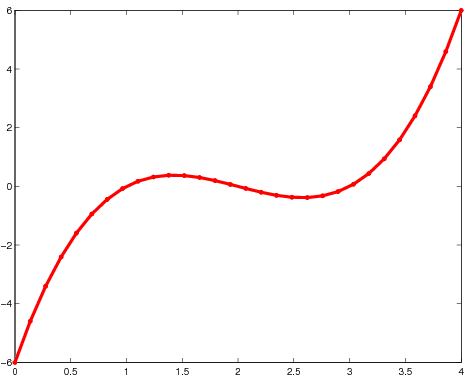
\includegraphics[width=0.6\textwidth]{figures/polynom_03_11} 
\end{center}

\end{frame}

%----------------------------
% Folie 
%----------------------------
\begin{frame}[fragile]\frametitle{Struktur von Function-Files}
Beispiel: 'myfunction.m'
\begin{lstlisting}
function [Out_1,..,Out_k] = myfunction(In_1,..,In_l)
% Beschreibung der Funktion
 ..
Out_1=..
 ..
Out_k=..
\end{lstlisting}
Soll keine Variable zurückgegeben werden, so besteht die erste Zeile aus
\begin{lstlisting}
function myfunction(In_1,..,In_k)
\end{lstlisting}

\alert{Wichtig:} Funktionsname = Dateiname.
\end{frame}
%----------------------------
% Folie 
%----------------------------
\begin{frame}[fragile]\frametitle{Function-Files}
\begin{itemize}
\item Funktionen sind mit Kommentaren zu versehen:
\begin{itemize}
\item (kurze) Beschreibung
\item Input-Argumente
\item Output-Argumente
\item Autor-Informationen und Datum
\end{itemize}
\item Variablen lokal, d.h.
\begin{itemize}
 \item Variablen des Workspace sind  nicht verfügbar.
\item definierte Variablen werden nicht im  Workspace gespeichert.
\end{itemize}
 
%oder kurz \alert{ \mcode{function myfile(In_1,...,In_k)}}.
\end{itemize}
\end{frame}

\subsection{Verwaltung von Dateien}

%----------------------------
% Folie 
%----------------------------
\begin{frame}[fragile]\frametitle{Priorität beim Programmaufruf}
Beispiel-Programmaufruf
\begin{lstlisting}
name
\end{lstlisting}

Testet ob,..
\begin{enumerate}
\item  \alert{Variable}
\item  \alert{Unterfunktion}. Eine
  Unterfunktion ist ein Programm/Funktion, die in derselben Datei wie der
  Aufruf steht.
\item  Programm im \alert{aktuellen Verzeichnis}.
\item  \textit{private function}.
\item  Programm im \alert{Suchpfad}. 
\end{enumerate}
Bei gefundenem Namen wird die Suche beendet.
\end{frame}

%----------------------------
% Folie 
%----------------------------
\begin{frame}[fragile]\frametitle{Suchpfad}

Der Suchpfad (Variable \mcode{path}) enthält Verzeichnisse in einer geordneten Liste.

\begin{itemize}
\item Abarbeitung erfolgt der Ordnung gemäss.
\item  Suchpfade hinzufügen:
\begin{lstlisting}
addpath <pfadname>
\end{lstlisting}
\item Suchpfade entfernen:
\begin{lstlisting}
rmpath <pfadname>
\end{lstlisting}
\end{itemize}
\end{frame}


%----------------------------
% Folie 
%----------------------------
\begin{frame}[fragile]\frametitle{Verwalten von m-Files}
\begin{itemize}
\item \alert{ \mcode{doc <name>}}\\ öffnet grafisches Hilfefenster zum jeweiligen Programm.
\item \alert{ \mcode{lookfor <name>}} \\ Suche nach \mcode{name} in den
  Kommentaren zu den Funktionen (auch: grafisches Hilfefenster).
\item  \alert{ \mcode{what}}\\ m-Files im aktuellen Verzeichnis.
\item  \alert{ \mcode{type <name>}}\\ Inhalt von \mcode{name.m} (Command Window).
\item  \alert{ \mcode{which <name>}}\\ absoluter Pfad der Datei, in dem die  Funktion
  \mcode{name} gespeichert ist. 
\item \alert{ \mcode{edit <name>}}\\ Ruft den Editor mit \mcode{name.m} auf.
\end{itemize}
\end{frame}








\section{Vektoren und Matrizen}



\subsection{Erzeugen von Vektoren}
%
% Slide: 
%
\begin{frame}[fragile]\frametitle{Vektoren I}
\begin{itemize}
\item Erzeugen 'per Hand'
\begin{lstlisting}
b = [1 2 4]
\end{lstlisting}
\begin{matlab}
b =
     1     2     4 
\end{matlab}

\item Abfragen der Einträge von $b$
\begin{lstlisting}
b(2)
\end{lstlisting}
\begin{matlab}
ans =      2 
\end{matlab}

Index $\equiv$ Position im Vektor\\

\alert{Achtung}: Indizes beginnen immer mit $1$!

\end{itemize}
\end{frame}

%
% Slide: 
%
\begin{frame}[fragile]\frametitle{Doppelpunkt - Notation}
\mcode{x:s:z} erzeugt einen Vektor der Form 
\[ (x,x+s,x+2s,x+3s, \ldots , z). \]
\begin{lstlisting}
>> a = 2:11
a =
 2  3  4  5  6  7  8  9  10  11

>> c = -2:0.75:1
c =
 -2.0000 -1.2500 -0.5000 0.2500 1.0000
\end{lstlisting}
\end{frame} 

%
% Slide: 
%
\begin{frame}[fragile]\frametitle{Vektoren II}
\begin{itemize}
\item \mcode{length(a)}\\ Länge des Vektors $a$ an.
\item \mcode{linspace(x1,x2,N)}\\ Vektor
\[ x1, x1+\frac{x2-x1}{N-1}, x1+2 \frac{x2-x1}{N-1}, \dots ,x2  \]
der Länge $N$.
\begin{lstlisting}
linspace(1,2,4)
\end{lstlisting}
\begin{matlab}
ans =
    1.0000    1.3333    1.6667    2.0000 
\end{matlab}

\item \mcode{logspace(x1,x2,N)}\\ wie \mcode{linspace}, nur logarith. Skalierung
\end{itemize}
\end{frame}

\subsection{Erzeugen von Matrizen}
%
% Slide: 
%
\begin{frame}[fragile]\frametitle{Erzeugen von Matrizen}
\begin{itemize}
\item Erzeugen 'per Hand'
\begin{lstlisting}
B = [1 3 4; 5 6 7]
\end{lstlisting}
\begin{matlab}
B =
     1     3     4
     5     6     7 
\end{matlab}

\item \mcode{eye(n,m)}\\ $(n \times m)$-EinheitsMatrix)
\begin{lstlisting}
eye(2,3)
\end{lstlisting}
\begin{matlab}
ans =
     1     0     0
     0     1     0 
\end{matlab}

($1$ auf der Hauptdiagonalen und 0 sonst).
\end{itemize}
\end{frame} 
%
% Slide: 
%
\begin{frame}[fragile]\frametitle{Erzeugen von Matrizen II}
\begin{itemize}
\item \mcode{zeros(n,m)}\\$(n \times m)$- Matrix mit $0$ als Einträge.
\item \mcode{ones(n,m)}\\$(n \times m)$- Matrix mit $1$ als Einträge.
\item Blockmatrizen
\begin{lstlisting}
C = [B zeros(2,2); eye(2,3) eye(2,2)]
\end{lstlisting}
\begin{matlab}
C =
     1     3     4     0     0
     5     6     7     0     0
     1     0     0     1     0
     0     1     0     0     1 
\end{matlab}

\alert{Achtung:} Matrizen in einer Zeile müssen dieselbe
Zeilenanzahl haben und Matrizen in einer Spalte dieselbe Spaltenanzahl.
\end{itemize}
\end{frame} 
%
% Slide: 
%
\begin{frame}[fragile]\frametitle{Erzeugen von Matrizen III}
\begin{itemize}
\item \mcode{repmat(A,n,m)}\\ Blockmatrix mit $(n \times m)$
  aus A bestehenden Blöcken
\begin{lstlisting}
D = repmat(B,1,2)
\end{lstlisting}
\begin{matlab}
D =
     1     3     4     1     3     4
     5     6     7     5     6     7 
\end{matlab}


\item \mcode{blkdiag(A,B)}\\ Blockdiagonalmatrix.
\item \mcode{diag(v,k)} \\Matrix der Größe $(n+|k|) \times
  (n+|k|)$ mit den Einträgen des Vektors $v$ auf der $k$-ten Nebendiagonalen. 
\end{itemize}
\end{frame}

\subsection{Manipulation von Matrizen}
%
% Slide: 
%
\begin{frame}[fragile]\frametitle{Beispiel-Matrizen}
\begin{itemize}
\item Überblick: \mcode{help gallery}
\item Beispiel
\begin{lstlisting}
E = gallery('moler',4)
\end{lstlisting}
\begin{matlab}
E =
     1    -1    -1    -1
    -1     2     0     0
    -1     0     3     1
    -1     0     1     4 
\end{matlab}

\item Hilfe zur Matrix 'moler' erhält man durch \mcode{help private/moler}
\item weitere Matrizen: \mcode{magic, hilb, vander}
\end{itemize}
\end{frame}
%
% Slide: 
%
\begin{frame}[fragile]\frametitle{Zugriff auf Matrizen}
\begin{columns}[c]%
\column{0.45\textwidth}%
\begin{lstlisting}[basicstyle=\tiny]
A = [1 2 3; 4 5 6; 7 8 9]
\end{lstlisting}%
\begin{matlab}
A =
     1     2     3
     4     5     6
     7     8     9 
\end{matlab}%
\end{columns}%
\begin{columns}[t,onlytextwidth]
\column{0.45\textwidth}
Abfragen eines Eintrags
\begin{lstlisting}
>> A(2,1)
ans =
     4
\end{lstlisting}
\column{0.45\textwidth}
Abfrage von Blöcken
\begin{lstlisting}
>> A(2:3,1:2)
ans =
     4     5     
     7     8     
\end{lstlisting}
\end{columns}
\begin{columns}[t,onlytextwidth]
\column{0.45\textwidth}
Abfrage einer Zeile
\begin{lstlisting}
>> A(2,:)
ans =
     4     5     6
\end{lstlisting}
\column{0.45\textwidth}
Abfrage mehrerer Zeilen
\begin{lstlisting}
>> A([1 3],:)
ans =
     1     2     3
     7     8     9
\end{lstlisting}
\end{columns}
\end{frame}
%
% Slide: 
%
\begin{frame}[fragile]\frametitle{Löschen}
\begin{columns}[c]%
\column{0.45\textwidth}%
\begin{lstlisting}[basicstyle=\tiny]
A = [ 1 2 3; 4 5 6; 7 8 9]
\end{lstlisting} 
\begin{matlab}
A =
     1     2     3
     4     5     6
     7     8     9 
\end{matlab}%
\end{columns}%
\begin{columns}[t]
\column{0.45\textwidth}%
Löschen einer Zeile
\begin{lstlisting}
>> A(2,:) = []
A =
     1     2     3
     7     8     9
\end{lstlisting}
\column{0.45\textwidth}%
Löschen von Spalten
\begin{lstlisting}
> A(:,[1 3]) = []
A =
     2
     5
     8
\end{lstlisting}
\end{columns}
\end{frame}

\subsection{Matrix- und Vektoroperationen}
%
% Slide: 
%
\begin{frame}[fragile]\frametitle{Matrizenoperationen}

Standard-Matrix Operationen \mcode{+,-,*}
\begin{lstlisting}
A = [1 2; 3 4]; B = 2*ones(2,2);
\end{lstlisting}
\begin{columns}[t]%
\column{0.25\textwidth}%
Multiplikation
\begin{lstlisting}
>>  A*B

ans =

     6     6
    14    14
\end{lstlisting}
\column{0.25\textwidth}%
Addition
\begin{lstlisting}
>> A+B

ans =

     3     4
     5     6
\end{lstlisting}
\column{0.25\textwidth}%
Subtraktion
\begin{lstlisting}
>> A-B

ans =

    -1     0
     1     2
\end{lstlisting}
\end{columns}
\end{frame}
%
% Slide: 
%
\begin{frame}[fragile]\frametitle{Andere Operatoren}
\begin{itemize}
\item \mcode{A\\\B}\\ Lösung $X$ von \mcode{A*X=B}. \\

\item \mcode{A/B}\\ Lösung $X$ von \mcode{X*A=B}.\\

\item \mcode{inv(A)}\\ Inverse von $A$.\\

\item \mcode{A'}\\ oder \mcode{ctranspose(A)}: komplex Transponierte von $A$. \\

\item \mcode{A.'}\\ oder \mcode{transpose(A)}: Transponierte von $A$. \\

\item \mcode{A^z}\\ (quadratische Matrizen) $\underbrace{A*A*\cdots *A}_{z-mal}$ \\

\item \mcode{size(A)}\\ Gr\"o{\ss}e einer Matrix $A$ . 
\end{itemize}
\end{frame}
%
% Slide: 
%
\begin{frame}[fragile]\frametitle{Punktnotation}
\begin{lstlisting}
A = [1 2; 3 4]; B = 2*ones(2,2);
\end{lstlisting}
\begin{itemize}
\item $C(i,j)=A(i,j)*B(i,j)$.
\begin{lstlisting}
>> C = A.*B
C =
     2     4
     6     8
\end{lstlisting}
\item $C(i,j)=A(i,j)/B(i,j)$.
\begin{lstlisting}
>> C = A./B
C =
    0.5000    1.0000
    1.5000    2.0000
\end{lstlisting}
\end{itemize}
\end{frame}
%
% Slide: 
%
\begin{frame}[fragile]\frametitle{Punktnotation}
\begin{itemize}
\item $C(i,j)=B(i,j)/A(i,j)$.
\begin{lstlisting}
>> C = A.\B
C =
    2.0000    1.0000
    0.6667    0.5000
\end{lstlisting}
\item $C(i,j)=A(i,j)^{B(i,j)}$
\begin{lstlisting}
>> C = A.^B
C =
     1     4
     9    16
\end{lstlisting}
\end{itemize}
\alert{Achtung:} Dimension von $A$ und $B$ gleich. \\Matrizen können durch
Skalare ersetzt werden, z.B. \mcode{ A.^2}.
\end{frame}
%
% Slide: 
%
\begin{frame}[fragile]\frametitle{Skalarprodukt}
\begin{itemize}
 \item Vektoren $a=(a_1, \dots ,a_n)$, $b=(b_1, \dots b_n)$ \\
\item Skalarprodukt: $a b^t$\\
\item Summe der Einträge von $a$: $(1, \dots , 1) a^t$\\
\end{itemize}
Beispiel:
\begin{lstlisting}
>> a=1:100; b=linspace(0,1,100);
>> a*transpose(b)
ans =
   3.3667e+03
>> ones(1,100)*transpose(a)
ans =
        5050
\end{lstlisting}  

\end{frame}


\end{document}